%\begin{savequote}[75mm]
% The idea that complex physical, biological or sociological systems can be exactly described by a few formulae is patently absurd. The construction of idealized representations that capture important stable aspects of such systems is, however, a vital part of general scientific analysis...
%\qauthor{Sir David Cox}
%\end{savequote}

\chapter{Background}
\label{chap:two}

This chapter lays the foundation for probabilistic modeling of neural
spike trains.  We start by introducing the language of generative
models, which allow us to formalize, in probabilistic terms, our
hypotheses about dynamics and low-dimensional structure.  The key
ingredients are latent variables that reflect the underlying state of
the system and conditional distributions that relate these variables
to the observed data.  Once we understand the basics of this language,
we can begin to articulate hypotheses about dynamical data in the form
of generative time series models.  Section~\ref{sec:motifs} enumerates
a few common motifs of time series modeling that will be used
throughout this thesis.  Finally, given a model and an observed spike
train, we can invert the model and reason about the posterior
distribution over latent variables using Bayesian inference algorithms
such as Markov Chain Monte Carlo and mean field variational inference,
which are introduced in Section~\ref{sec:inference_algorithms}.  At
the end of this chapter, we will have the basic foundation necessary
to start looking for structure in neural data. The rest of the thesis
will build upon this foundation by developing more sophisticated
models and increasingly efficient inference algorithms, and by putting them to
use on real neural recordings.

\section{Generative Probabilistic Models}
\label{sec:generative_models}
Generative probabilistic models tell a story of how data comes to be. 
While this story never captures every physical detail, it serves as an 
idealized version, capturing the essence of the system. For example, when
modeling a neural spike train, we will ignore the states of individual ion 
channels and the nonlinear dynamics of membrane potential and instead 
characterize the instantaneous \emph{firing rate} of a neuron --- the 
probability that a neuron spikes at any moment in time. 

As a simple illustration, consider the following generative
process. Suppose a neuron has two states, an \emph{up} state and a
\emph{down} state. In the \emph{up} state, it spikes at a high
rate, say 100Hz, and in the \emph{down} state it fires less frequently, say at 10Hz.
Assume that every 50ms the neuron flips a coin to decide its new state
and then fires a random number of spikes according to the
firing rate associated with that state. For the sake of simplicity, 
assume the precise spike times are uniformly distributed over the 50ms
interval. Once the interval has elapsed, the neuron
flips another coin and its rate immediately changes to reflect its new
state.   Our goal is to infer the latent state of
the neuron given the observed spikes.

\begin{figure}[t]
\centering%
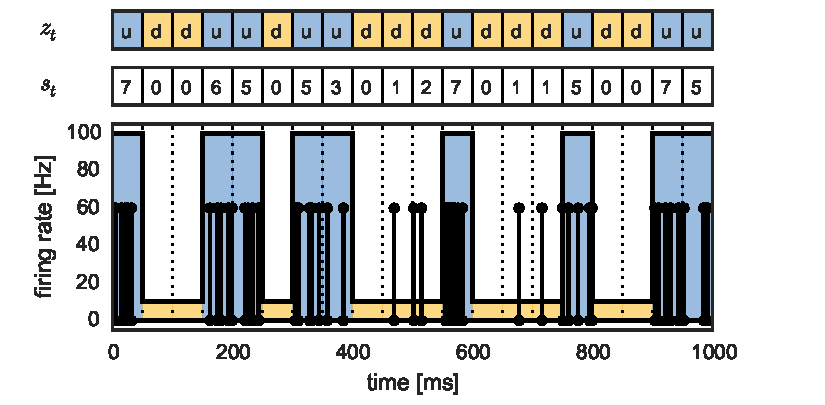
\includegraphics[width=5.5in]{figures/ch2/figure1} 
\caption[Simple neuron with up and down states]{A simple neuron that
  randomly switches between an \textit{up} and a \textit{down} state
  every 50ms. Here, time bins are colored blue and yellow depending on
  the latent state,~$z_t$. Each state has an associated firing rate from
  which a Poisson number of spikes,~$s_t$, is drawn. Precise spike
  times are uniformly distributed over the 50ms interval.}
\label{fig:updown}
\vspace{-0.5cm}
\end{figure}


Clearly, this generative story contains many simplifying assumptions
and omits a great amount of detail. In addition to assuming that
spiking is adequately captured by firing rates, the notion that a
neuron has only two firing rates and that it randomly switches between
them is a gross simplification. Nevertheless, this very
simple model captures patterns of spiking that have been observed
in actual experiments \citep{cowan1994spontaneous, shu2003turning}. 

\sloppy We can formalize this generative story with a probabilistic
model that specifies a distribution over latent states and observed
spike counts. Let~$s_t \in \naturals$ denote the number of spikes
counted in the~$t$-th time bin, and~$z_t \in \{\textit{up},
\textit{down}\}$ denote the corresponding state of the neuron. The
assumption that states are drawn from a coin flip corresponds to the
prior distribution, ${z_t \sim \distDiscrete(\bpi)}$, where~${\bpi =
  [\pi_{\textit{up}}, \pi_{\textit{down}}]}$ is a nonnegative vector
that sums to one and specifies the probability of \textit{up} and
\textit{down} states.\footnote{The notation~${z \sim
    \mathrm{P}(\theta)}$ means that the random variable~$z$ is sampled
  from (or distributed according to) the distribution~$P$, which is
  parameterized by~$\theta$. When we write~${\mathrm{P}(z \given
    \theta)}$ we refer to the density (assuming it exists)
  of~$\mathrm{P}$ evaluated at~$z$.  A list of commonly used
  distributions and their densities is given in Appendix~\ref{app:A}.}
Implicitly, we have assumed that~${\bpi=\big[\tfrac{1}{2},
    \tfrac{1}{2} \big]}$, though this need not be the case.  We
previously said that the neurons fire a random number of spikes
according to their state-dependent firing rate; now we will formalize
this by assuming,~${s_{t} \sim \distPoisson(\lambda_{z_t} \cdot \Delta
  t)}$, where ${\Delta t = 0.05\text{s}}$, ${\lambda_{\textit{up}} =
  100\,\text{spikes/s}}$, and ${\lambda_{\textit{down}} =
  10\,\text{spike/s}}$.

Figure~\ref{fig:updown} shows a neural spike train sampled from this
generative model. The time bins are colored blue or yellow depending
on whether the neuron is in the \textit{up} or \textit{down} state,
respectively.  The precise spike times are denoted by black vertical
lines with circular endpoints. Above, the vector of observed spike
counts, ${\bs = \big[s_1, \ldots, s_T \big]}$, and the vector of
latent states,~${\bz = \big[z_1, \ldots, z_T \big]}$, are shown.  We
will use this notation throughout the thesis: bold symbols like~$\bs$
will denote arrays of random variables; lowercase bold symbols will
typically denote vectors.

The generative procedure defines the \emph{likelihood} of any given
set of observed spike counts and corresponding latent states. This can
be written as a conditional distribution where the state probabilities
and firing rates are given. We have,
\begin{align}
  \label{eq:lkhd_chain_rule}
  p(\bs, \bz \given \bpi, \blambda) 
  &= p(\bz \given \bpi) \, p(\bs \given \bz, \blambda) \\
  \label{eq:lkhd_factorized}
  &= \prod_{t=1}^T p(z_t \given \bpi) \, p(s_t \given \lambda_{z_t}) \\
  \label{eq:lkhd_factorized_forms}
  &= \prod_{t=1}^T \distDiscrete(z_t \given \bpi) \, \distPoisson(s_t \given \lambda_{z_t} \cdot \Delta t).
\end{align}
Since~$\Delta t$ is a constant, we do not include it as a random
variable in the joint distribution or explicitly condition on it.

The probabilistic model specifies the particular factorization of the
likelihood implied by the generative story.
Eq.~\ref{eq:lkhd_chain_rule} applies the product rule of
probability, and reflects the assumptions that~$\bz$ depends only on~$\bpi$
and~$\bs$ depends only on~$\bz$ and~$\blambda$. 
In going from \eqref{eq:lkhd_chain_rule} to
\eqref{eq:lkhd_factorized}, we have asserted that the latent
states~$z_t$ and~$z_{t'}$ are conditionally independent given~$\bpi$,
and that the spike counts~$s_{t}$ and~$s_{t'}$ are conditionally
independent given their corresponding latent states and firing rates. This conditional
independence assumption, which was implicit in the generative story,
becomes explicit when we factor the likelihood into a product over
time bins.  Eq.~\ref{eq:lkhd_factorized_forms} specifies the
functional form of the conditional distributions.  When we hypothesize
relationships between different variables, we are making assertions
about the factorization and the form of the likelihood.  In
Section~\ref{sec:motifs}, we explore different patterns of conditional
dependence that provide the building blocks of models for dynamic
data.

So far, we have assumed that the firing rates and state probabilities are known, but in practice 
this is a bit unreasonable. To complete the probabilistic model, we need 
to combine the likelihood function with a \emph{prior distribution} that 
captures our uncertainty about these parameters. 
For example, a more reasonable hypothesis is that neurons have 
two firing rates, and while we do not know their exact values, we can 
specify a distribution over them,~$p(\blambda)$. Similarly, we may not know 
the exact probability of each state,~$\bpi$, but perhaps we can specify 
a prior,~$p(\bpi)$, that captures our intuition that the states should
be equally likely \emph{a priori}.
Putting this all together, we can now write down the \emph{joint
  distribution} of our probabilistic model --- the
product of the likelihood and the prior distributions:
\begin{align}
  \label{eq:full_joint}
  p(\bs, \bz, \bpi, \blambda \given \alpha, \beta, \gamma) 
  &= p(\bs, \bz \given \bpi, \blambda) \,
  p(\bpi \given \gamma) \, 
     p(\blambda \given \alpha, \beta).
\end{align}

When constructing a probabilistic model, we express these prior
intuitions and simultaneously make inference easier by using
\emph{conjugate} prior distributions.


% Prior distributions on parameters
\subsubsection{Conjugate Prior Distributions}
A conjugate prior ensures that the conditional distribution of a
parameter, given the data, will have a tractable form.  Specifically,
the conditional distribution will have the same form as the prior.
For example, take the parameter,~$\lambda_{\textit{up}}$. If we look
at the likelihood as a function of~$\lambda_{\textit{up}}$ and ignore
terms that do not depend on this parameter, we have,
\begin{align*}
  p(\bs, \bz \given \bpi, \blambda)
  &\propto \prod_{t=1}^T \left[
    \distPoisson(s_t \given \lambda_{\textit{up}} \cdot \Delta t)
    \right]^{\bbI[z_t = \textit{up}]} \\
  &\propto \prod_{t=1}^T \left[
    \lambda_{\textit{up}}^{s_t} \,
    e^{-\lambda_{\textit{up}} \cdot \Delta t}
    \right]^{\bbI[z_t = \textit{up}]} \\
  &=
  \lambda_{\textit{up}}^{s_{\textit{up}}} \,
  e^{-\lambda_{\textit{up}} \cdot t_{\textit{up}}},
\end{align*}
where
\begin{align*}
  s_{\textit{up}} &= \sum_{t=1}^T s_t \cdot \bbI[z_t = \textit{up}], \\
  t_{\textit{up}} &= \sum_{t=1}^T \Delta t \cdot \bbI[z_t = \textit{up}],
\end{align*}
and~$\bbI[x]$ is an indicator function that equals one if~$x$ evaluates to true
and equals zero otherwise.

%This likelihood is conjugate with a gamma prior,
Now consider a gamma prior distribution,
\begin{align*}
  p(\lambda_{\textit{up}} \given \alpha, \beta)
  &= \distGamma(\lambda_{\textit{up}} \given \alpha, \beta) \\
  &\propto \lambda_{\textit{up}}^{\alpha - 1} \,
  e^{-\lambda_{\textit{up}} \cdot \beta}.
\end{align*}
The conditional distribution over~$\lambda_{\textit{up}}$ given the
observed spike counts, the latent states, and the prior is
proportional to the likelihood times the prior. This simplifies to,
\begin{align*}
  p(\lambda_{\textit{up}} \given \bs, \bz, \alpha, \beta)
  &\propto p(\bs, \bz \given \bpi, \blambda) \,
  p(\lambda_{\textit{up}} \given \alpha, \beta) \\
  &\propto \lambda_{\textit{up}}^{s_{\textit{up}} + \alpha - 1} \,
  e^{-\lambda_{\textit{up}} (t_{\textit{up}} +\beta)} \\
  &\propto \distGamma(\lambda_{\textit{up}} \given
  s_{\textit{up}} + \alpha, \,
  t_{\textit{up}} + \beta).
\end{align*}
Since both the prior and the the conditional distribution
over~$\lambda_{\textit{up}}$ are in the gamma family, we say gamma
prior is conjugate with this product-of-Poissons likelihood.
Moreover, the parameters of conditional distribution only depend
on~$\bs$ and ~$\bz$ through simple \emph{sufficient
  statistics},~$s_{\textit{up}}$ and~$t_{\textit{up}}$. A Dirichlet
prior distribution on the state probability, ~${\distDirichlet(\bpi
  \given \gamma)}$, is similarly conjugate with the
product of discrete densities in the likelihood that links~$\bpi$ and~$\bz$.  In
fact, conjugate priors exist for all likelihoods in the
\emph{exponential family}. These ideas are thoroughly discussed in
standard Bayesian statistics and machine learning textbooks
like~\citet{Gelman13, murphy2012probabilistic}.


% Latent variables (states at each time)
% Parameters rates associate with each state
\paragraph{Latent Variables, Parameters, and Hyperparameters}
As our models become increasingly complicated, we will often distinguish
between the different types of random variables. The states,~$\bz$,
are called \emph{local latent variables} because there is one for each
data point.  The unknown latent state probability and the
firing rates,~${ \{\bpi, \blambda\} }$, are either called \emph{parameters} or
\emph{global latent variables} because their dimension is fixed. The
remaining values,~${\{ \alpha, \beta, \gamma \} }$,
are called \emph{hyperparameters}. These are constants that we set
prior to performing inference.  Typically, these can be tuned by
cross-validation, or simply set based on intuition and physical
constraints. For conciseness, we will refer to the set of
all parameters as~$\btheta$ and the set of hyperparameters
as~$\boldeta$.


\subsection{Representations of Spike Trains}
% Notation for sets of spike times or spike count matrices
One of the first decisions we must make is how to
represent our data. In this thesis we will focus solely on modeling
spike trains, which are sequences of discrete events in time. These
spike trains typically come from spike sorting algorithms applied to
extracellular recordings from multi-electrode arrays
\citep{lewicki1998review} or from
deconvolution algorithms applied to optically recorded calcium
fluorescence traces \citep{pnevmatikakis2016simultaneous,
  vogelstein2010fast}. Reducing the data to a set of spike times often 
results in enormous compression. Rather than considering electrode 
potentials, which may be sampled at upwards of 10kHz, or calcium 
fluorescence traces, which are highly autocorrelated due to the relatively 
slow dynamics of calcium concentration in cells, we only consider 
the times of action potentials.

% While this thesis treats the spike trains as given, it is also possible to
% work directly with the observed extracellular recordings or calcium
% fluorescence and treat the spike train as a latent variable.  Then,
% the spike train must be inferred along with the rest of the model's
% latent variables and parameters, cf. \citep{pillow2013model}. As we just 
% mentioned, this will typically incur a substantial cost, but it may be 
% worthwhile if there is considerable uncertainty in the spike timing 
% and if precise timing is important to the overarching model.

The most general representation 
of a spike train is a set of real-valued times for each neuron.
In Figure~\ref{fig:updown}, this corresponds to the temporal locations of
each black spike.
When there is more than one neuron, we have a set of
\emph{marked} spike times, which we call,
\begin{align*}
  \mcS = \left \{ (s_m, c_m) \right \}_{m=1}^M \subset [0, T] \times \{1, \ldots, N\}.
\end{align*}
Each member of this set consists of a real-valued spike time~$s_m$ in
the interval~$[0, T]$, and an integer,~$c_m \in \{1, \ldots, N\}$,
that specifies the index of the cell that generated this spike. $M$ is 
the total number of spikes on all neurons.

% In the working example of a neuron with an \emph{up} and \emph{down}
% state there is only one neuron ($N=1$), so the cell markers would be
% trivially equal to~$c_m=1$.
This continuous-time representation is
warranted when the temporal resolution of the data is considerably
higher than the timescale of typical action potentials. For example,
multi-elecrode arrays typically have sampling intervals of~$0.1$ms or
smaller, whereas the width of action potentials is on the order
of~$1$ms. This allows us to specify the spike time as an effectively
real-valued number.  
% Calcium imaging methods typically have much lower temporal
% resolution and are often sampled at lower rates, but by deconvolving
% spike trains it may be possible to obtain effectively higher
% resolution than the raw data affords.


Sets of discrete events like these are typically modeled as realizations
of a \emph{marked point process} \citep{daley2003introduction1}. Such a
process is defined by its nonnegative firing rates\footnote{In the
  point process literature, these firing rates are called
  \emph{conditional intensity functions}.},
${\{\lambda_n(t \given \mcH_t)\}_{n=1}^N}$, where $\mcH_t$ captures
the history of the process through time~$t$. For example, the history
may include the previous spikes,~${\mcH_t = \{(s_m, c_m): s_m < t\}}$,
as well as some external covariates.  If we consider a small time
window,~${[t, t+\Delta t)}$, and take the limit as~$\Delta t$
approaches zero,~${\lambda_n(t \given \mcH_t) \cdot \Delta t}$ is the
expected number of spikes fired by neuron~$n$ in the
window~${[t, t+\Delta t)}$.  
% Our goal is then to specify flexible and
% interpretable conditional intensity
% functions. 

The limiting perspective on the conditional intensity functions
suggests an alternative, discrete-time representation.  Rather than
modeling a set of continuous spike times and conditional firing rates,
we may instead represent a spike count matrix,~$\bS$, and the
corresponding rate matrix,~$\bLambda$, where,
\begin{align*}
  \bS &= 
        \begin{bmatrix}
          s_{1,1} & \cdots & s_{1,N} \\
          & & \\
          \vdots  &        & \vdots  \\ 
          & & \\
          s_{T,1} & \cdots & s_{T,N}
        \end{bmatrix}, 
  & & &
  \bLambda &= 
        \begin{bmatrix}
          \lambda_{1,1} & \cdots & \lambda_{1,N} \\
          & & \\
          \vdots  &        & \vdots  \\ 
          & & \\
          \lambda_{T,1} & \cdots & \lambda_{T,N}
        \end{bmatrix}.
\end{align*}
Here,~${s_{t,n} \in \naturals}$ denotes the number of spikes fired in
the~$t$-th time bin by the~$n$-th neuron, and~${\lambda_{t,n} \in \reals_+}$ denotes 
the corresponding firing rate. Sometimes, the effects we
are interested in studying occur at relatively slow time scales, so
discretizing may provide valuable compression while retaining most of
the relevant information. For example, if we are studying neural
dynamics on the order of minutes, then simply knowing how many spikes
occurred each second may provide most of the relevant information, while
precise, millisecond-resolution spike timing may be superfluous.

However, the primary reason to discretize spike times into a matrix of
counts is that the statistics and machine learning community has
developed a much broader set of models for matrices than for sets of
continuous time events.  In the next section, we will explore a number
of common modeling motifs that can be applied to time series data
represented as matrices, and many of the chapters of this thesis will
focus on extending these motifs in novel ways.


\section{Motifs of Time Series Models}
\label{sec:motifs}
The art of probabilistic modeling lies in balancing two conflicting
concerns: our model should capture as much of the relevant structure
in the data as possible, drawing on our intuition and our existing
knowledge of the system, yet at the same time we wish to limit the
complexity of the model so that we may perform inference
efficiently. One way to balance these goals is to compose our model
out of common, well-studied motifs.

Motifs correspond to factorizations of probabilistic models.  To
visualize these motifs, we represent the probabilistic model in the
form of a directed acylcic graph. Each node in the graph corresponds
to a random variable, and shaded nodes indicate which variables are
observed. The edges represent conditional dependencies. For example,
in the mixture model shown in Figure~\ref{fig:motifs}, the spike
count~$s_2$ has incoming edges from the corresponding latent
state~$z_2$ and the firing rates,~$\blambda$.  Thus, the joint
probability distribution contains the factor,~$p(s_2 \given z_2,
\blambda)$. Since the graph is directed and acyclic, we read off
the factors starting with the root nodes,~$p(\bpi)$ and~$p(\blambda)$,
and ending with the leaf nodes, ~$p(s_t \given z_t, \blambda)$. In
this way, the graph captures the factorization of the joint
probability distribution and specifies a particular subset of all
possible joint distributions over this set of variables.

The edges of the graph do not, however, specify the type of the random
variable or functional form of the factors. For example, a node may
indicate either a discrete or a continuous random variable, and an
edge may indicate an arbitrary form of dependence, like a linear 
relationship.
In this way, two models may share the same graph but have
fundamentally different interpretations. This is true of mixture
models and factor analysis models shown in Figure~\ref{fig:motifs}.
Some patterns of factorization, types, and dependencies are used
over and over again and form the
building blocks for more complex models.
Next, we discuss a few of the common motifs shown in Figure~\ref{fig:motifs}.

\begin{figure}[t]
  \centering%
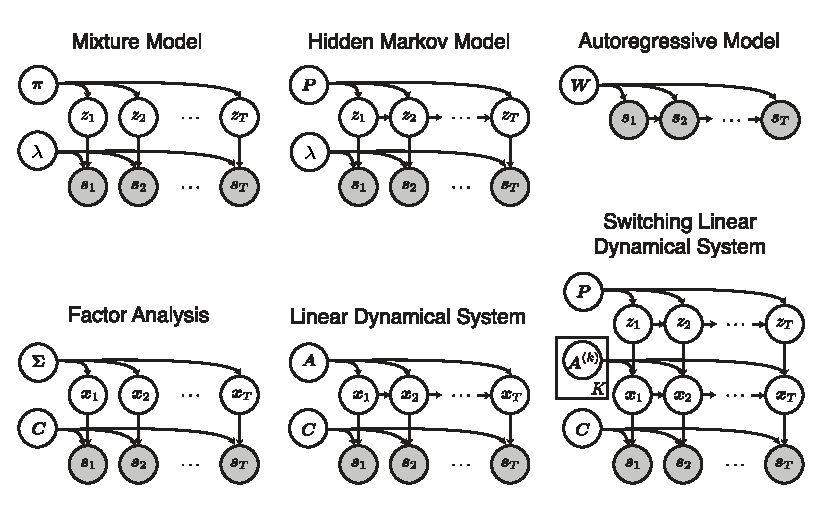
\includegraphics[width=5.5in]{figures/ch2/figure2b} 
\vspace{-.25in}
\caption[Motifs of time series models]{Motifs of time series models.
  By introducing conditional dependencies and layers of random
  variables, we construct models that reflect sophisticated hypotheses
  about the structure underlying the data.  See
  Section~\ref{sec:motifs} for detailed description.}
\label{fig:motifs}
\end{figure}


\paragraph{Mixture Models}
% Discrete latent states
Our working example from Section~\ref{sec:generative_models} is an
instance of a simple mixture model.  The firing rate assumes
only two values, and the observed spike counts are a mixture of counts
drawn from the \textit{up} state and counts from the \textit{down}
state. We can easily extend this to populations of neurons and
mixtures of more than two states.  Suppose there are now~$K$ states,
such that~${z_t \in \{1, \ldots, K\}}$. Furthermore, we generalize the
rates~$\lambda_{\textit{up}}$ and~$\lambda_{\textit{down}}$, to
vectors of rates, one for each neuron and state.  In a slight abuse of
notation, let~${\blambda_k = [\lambda_{k,1}, \ldots, \lambda_{k,N}]}$
denote a vector of rates in which $\lambda_{k,n}$ is the firing rate of
the~${n\text{-th}}$ neuron in state~$k$.

In a mixture model, the latent states are discrete, the time bins are
conditionally independent, and the dependence of~$s_t$ on~$z_t$
and~$\blambda$ is linear.  To see the latter claim, note that that the
instantaneous firing rate of neuron~$n$ can be written,
${\sum_{k=1}^K \bbI[z_t=k] \cdot \lambda_{k,n}}$. These three
properties suggest multiple dimensions along which the mixture model
may be generalized.

%We can write the full rate
%matrix,~$\bLambda$, as the outer product of a ~${T \times K}$
%indicator matrix,~$\bZ$, and an~${N \times K}$ rate
%matrix,~$\bC$. Let~$\be_k$ denote a length-$K$ column vector that is all zero
%except for a single one in the~$k$-th position.
%Then,~${\bLambda = \bZ \bC^\trans}$, where,
%\begin{align}
%  \bZ = 
%        \begin{bmatrix}
%          - & \be_{z_1}^\trans & - \\
%            &                  &   \\
%            &  \vdots          &   \\
%            &                  &   \\
%          - & \be_{z_T}^\trans & - 
%        \end{bmatrix}, 
%  \qquad
%  \bC = 
%        \begin{bmatrix}
%          | &  & | \\
%          \blambda_1 & \cdot \cdot & \blambda_K \\
%          | &  & | 
%        \end{bmatrix}.
%\end{align}
%Now that we have framed the mixture model as a simple factorization of 
%the rate matrix, a number of connections and extensions become clear.

\paragraph{Hidden Markov Models}
First, let's address the conditional independence of time bins in the
mixture model. According to this model, the distribution over latent
states factors into a product,~${p(\bz \given \bpi) = \prod_t p(z_t
  \given \bpi)}$.  This clearly ignores the temporal dynamics of
neural data. Instead, we may hypothesis that latent states obey
Markovian dynamics,
\begin{align*}
  p(\bz \given \bpi^{(0)}, \bP) &= p(z_1 \given \bpi^{(0)}) \prod_{t=2}^T p(z_t \given z_{t-1}, \bP) \\ 
  &= \distDiscrete(z_1 \given \bpi^{(0)}) \prod_{t=2}^T \distDiscrete(z_t \given \bpi^{(z_{t-1})}),
\end{align*}
where~$\bpi^{(0)} \in [0,1]^K$ is a discrete probability distribution over
initial states, and
\begin{align*}
  \bP &=
        \begin{bmatrix}
          \text{---} &  \bpi^{(1)}  & \text{---} \\
            &  \vdots &   \\
          \text{---} &  \bpi^{(K)}  & \text{---}
        \end{bmatrix},
\end{align*}
is a~${K \times K}$ transition matrix where the
row,~${\bpi^{(k)} \in [0,1]^K}$, specifies a discrete conditional
distribution over~$z_t$ given~${z_{t-1}=k}$.  This is known as a
hidden Markov model (HMM) \citep{baum1966statistical,
  rabiner1989tutorial}, and the corresponding graphical model is shown
in Figure~\ref{fig:motifs}. Chapter~\ref{chap:seven} studies some of
the challenges involved in selecting the number of states,~$K$, in a
nonparametric way.

\paragraph{Autoregressive Models}
% Autoregressive observations
In an HMM, correlations in spike counts from one bin to the next arise from 
correlations in the underlying latent states. Alternatively, we may directly 
model the rate as a function of previous spike counts. For example, consider 
an autoregressive model with linear dynamics,
\begin{align}
  \label{eq:ar_model}
  \lambda_{t,n} &= \sum_{m=1}^N \sum_{d=1}^D w_{m \to n}^{(d)} \cdot s_{t-d, m}.
\end{align}
The weight,~$w_{m \to n}^{(d)}$, specifies the influence that spikes
on neuron~$m$ have on the rate of neuron~$n$ at an offset of~$d$ time bins
in the future. 
Unlike the HMM, which has an
autoregressive model for latent states, here the
autoregression governs the rates directly.
Moreover, this
autoregressive model sums over the spike counts of all neurons over
the past~$D$ time bins, allowing delayed interactions.
Figure~\ref{fig:motifs} shows the graph structure of an autoregressive model
in the special case that~$D=1$.

In continuous time, autoregressive interactions like these are the
basis of the Hawkes process \citep{Hawkes-1971}, a mutually-excitatory
point process. Chapter~\ref{chap:three} will study these models 
in great detail, and Chapter~\ref{chap:four} will extend the Hawkes
process inference algorithms to their discrete time counterparts.

Since the firing rates must be nonnegative, the weights must be as
well.  That is,~$w_{m \to n}^{(d)} \in \reals_+$.  This implicitly
instantiates the hypothesis that interactions between spikes on one
neuron and the rate of another is always excitatory~---~a spike can
never decrease the future firing rate.  While this is not the most
biologically realistic model given our knowledge of excitatory and
inhibitory synapses, it is important to remember that this is simply a
descriptive model of firing rate dynamics, and it does not necessarily
map onto physical synaptic connections. As we will show, the weights
inferred by this type of excitatory autoregressive model can still
provide useful insight into the structure of neural activity.

\paragraph{Nonlinear Autoregressive Models}
In order to capture both excitatory and inhibitory autoregressive weights,
we need to introduce a nonlinear function that ensures a nonnegative firing 
rate. Specifically, assume that,
\begin{align*}
  \psi_{t,n} &= \sum_{m=1}^N \sum_{d=1}^D w_{m \to n}^{(d)} \cdot s_{t-d,m}, \\
  \lambda_{t,n} &= g \left( \psi_{t,n} \right).
\end{align*}
The nonlinear function~${g(\cdot): \reals \to \reals_+}$ maps a real
valued ``activation,''~$\psi_{t,n}$, into a nonnegative firing
rate,~$\lambda_{t,n}$. 
%It is common to use an exponential or a
%sigmoidal nonlinearity. 
In this formulation, the weights may be either
positive or negative to reflect either excitatory or inhibitory
interactions, respectively.  In computational neuroscience, this is
often called a generalized linear model (GLM) \citep{Paninski-2004,
  Truccolo-2005, Pillow-2008}, since the linear-nonlinear cascade
that links spike history to firing rate is an instance of the
GLM commonly used in statistics \citep{nelder1972generalized}.
Chapter~\ref{chap:five} combines these nonlinear autoregressive models
with prior distributions on the underlying network and derives
efficient Bayesian inference algorithms to fit them to data.

\paragraph{Factor Models}
HMM's introduced dynamics to the mixture model and nonlinear
autoregressive models generalized the linear functional dependence.
Factor models generalize the discrete nature of the random variables
with a continuous analogue. For example, consider a model in which the
discrete variable~${z_t \in \{1, \ldots, K\}}$ is replaced by a
discrete probability distribution~${\bpi_t \in [0,1]^K}$. The rate
is then a nonnegative combination,
\begin{align*}
  \lambda_{t,n} &= \sum_{k=1}^K \pi_{t,k} \cdot \lambda_{k,n}
\end{align*}
This is naturally interpreted as a \emph{mixed membership model} in
which the rates at each time bin derive from a mixture of discrete
latent states with mixing weights~$\bpi_t$. In text modeling, this motif
is the basis of the latent Dirichlet allocation (LDA)
model~\citep{blei2003latent}.

Alternatively, we may replace the discrete latent state with a continuous
one,~$\bx_t \in \reals^K$. As in the nonlinear autoregressive model,
we can retain the linear form and introduce an elementwise nonlinearity
to ensure nonnegative firing rates:
\begin{align*}
  p(\bx) &= \prod_{t=1}^T \distNormal(\bx_t \given \bzero, \bSigma), \\
  \psi_{t,n} &= \sum_{k=1}^K x_{t,k} \cdot c_{k,n}, \\
  \lambda_{t,n} &= g(\psi_{t,n}).
\end{align*}
Here,~$c_{k,n}$ is an entry in the real valued matrix~$\bC \in
\reals^{K \times N}$, and~${\bSigma = \diag \left([ \sigma^2_1,
    \ldots, \sigma^2_K ] \right)}$.  This corresponds to a factor
analysis model. Unlike standard factor analysis, however, here the
observations are discrete spike counts rather than Gaussian
observations.

\paragraph{Linear Dynamical Systems}
In the same way that HMM's extend mixture models with temporal
dynamics, linear dynamical systems (LDSs) extend factor models with
linear autoregressive dynamics in the latent state.  We simply replace
the prior on~$\bx$ with a model of the form,
\begin{align*}
  p(\bx) &= \distNormal(\bx_1 \given \bzero, \bSigma) \prod_{t=2}^T \distNormal(\bx_t \given \bA \bx_{t-1}, \bSigma),
\end{align*}
where~$\bA \in \reals^{K \times K}$ specifies the linear dynamics of
the latent state.  The elementwise nonlinear mapping from latent
states to firing rates is the same as in the factor model, but now the
linear autoregressive nature of the dynamics induces correlations in
spike counts from one time bin to the next.

% Switching LDS

\paragraph{Hierarchical Extensions}
These motifs --- continuous and discrete latent states, linear autoregressive 
dynamics, and nonlinear link functions --- provide a foundation for 
constructing probabilistic models for spike trains. Atop this foundation,
we may layer additional random variables reflecting hypotheses about shared 
structure. For example, a switching linear dynamical system, shown in Figure~\ref{fig:motifs}
and studied in Chapter~\ref{chap:eight},
combines discrete \emph{and} continuous latent states \citep{murphy2012probabilistic, fox2009bayesian}. 
Likewise, Chapters~\ref{chap:three}, \ref{chap:four},
and~\ref{chap:five} consider structured prior distributions on 
the weights of autoregressive models, and Chapter~\ref{chap:seven} considers 
nonparametric Bayesian priors on the number of states in an HMM. Once the 
dynamics model has been specified, it is easy to test a variety of hypotheses
about hierarchical structure. In order to fit these models, however, we need 
efficient inference algorithms that capitalize on the compositional structure 
of the model.


% Inference in this model is not quite as straightforward as in the
% Gaussian case. In Chapter~\ref{chap:discussion}, we discuss some ways
% in which the ideas of Chapter~\ref{chap:nonlinear_hawkes} could be
% extended to

\section{Bayesian Inference}
\label{sec:inference_algorithms}
Given an observed spike train, our goal is to compute the posterior
distribution over latent variables,~$\bz$, and parameters,~$\btheta$,
of the model.  For example, in an HMM the latent variables are 
the dynamic latent states and the parameters
are~${\btheta = \{\bP, \blambda\}}$, the transition matrix and the
firing rates for each latent state. Bayes' rule relates the posterior
distribution to the joint distribution of our probabilistic model,
\begin{align}
  \label{eq:bayes_rule}
  p(\bz, \btheta \given \bs) 
  &= \frac{p(\bs, \bz, \btheta)}{p(\bs)} 
   = \frac{p(\bs, \bz, \btheta)}{\int p(\bs, \bz, \btheta) \, \mathrm{d}\bz \, \mathrm{d}\btheta} .
\end{align}
Unfortunately, the denominator in Eq.~\ref{eq:bayes_rule} involves an 
integral that is intractable for 
all but the simplest models. Instead, we must resort to approximate 
algorithms like Markov Chain Monte Carlo (MCMC) and mean field variational 
inference. We will briefly describe each of these in turn.

\subsection{Markov Chain Monte Carlo}
Markov Chain Monte Carlo (MCMC) algorithms are a workhorse of modern
machine learning, and many texts are devoted to the subject
\citep[e.g.][]{geyer1992practical, gilks2005markov, robert2013monte}.
The fundamental idea is to generate a collection of samples from the
posterior distribution and use them to estimate expectations.
Specifically, given a set of samples,
\begin{align*}
  \left \{ \big(\bz^{(1)}, \btheta^{(1)} \big), 
           \ldots, 
           \big(\bz^{(L)}, \btheta^{(L)} \big) 
  \right\},
\end{align*}
where
\begin{align*}
  \bz^{(\ell)}, \btheta^{(\ell)} &\sim p(\bz, \btheta \given \bs),
\end{align*}
we can form a Monte Carlo estimate of the expectation of a function~$f(\bz, \btheta)$
with respect to the posterior,
\begin{align*}
  \bbE_{p(\bz, \btheta \given \bs)} \left[ f(\bz, \btheta) \right] 
  &\approx \frac{1}{L} \sum_{\ell = 1}^L f \big(\bz^{(\ell)}, \btheta^{(\ell)} \big).
\end{align*}
When the samples are independently drawn from the posterior, the strong 
law of large numbers states that the Monte Carlo estimate converges to 
the true expectation almost surely, implying that these Monte Carlo
estimates are unbiased. Moreover, if the function~$f$ is real-valued, 
the variance of the Monte Carlo estimator scales as~$\mcO(L^{-1})$
regardless of the dimension of~$\bz$ and~$\btheta$.


To collect these samples, we design a Markov chain to stochastically
explore the space of latent variables and parameters.  
%For notational clarity, we will now refer to these collectively as~${\bx = (\bz, \btheta)}$.  
The chain iteratively samples a new state according to its transition
operator,~${\mcT \big((\bz, \btheta) \to (\bz', \btheta') \big)}$,
which specifies the probability of transitioning from state~${(\bz,
  \btheta)}$ to state~${(\bz', \btheta')}$.  Each state the Markov
chain visits is taken as a sample. If we design the Markov chain
appropriately, we guarantee that the transition operator will
asymptotically visit states according to their posterior probability.

When states are sampled with a Markov chain, it is no longer true that
the samples are independent. In fact, the transition operator often
leads to relatively local updates, which in turn lead to
autocorrelation in the sequence of samples. This does not affect the
bias of the Monte Carlo estimate, but it does affect the constant in the
asymptotic~$\mcO(L^{-1})$ convergence rate. However, in addition to
the increased variance, MCMC algorithms also suffer from a transient
bias due to the fact that the initial state is not drawn from the
posterior distribution (we would not be using MCMC if we could sample
from the posterior directly). Fortunately, the transient bias of the
Monte Carlo estimator also decays as~$\mcO(L^{-1})$. Since the mean
squared error of an estimator is equal to its variance plus its bias
squared, and since both variance and bias scale inversely with~$L$,
the asymptotic effect of the transient bias is insignificant compared
to that of the variance.

The critical property of our Markov chain is that, asymptotically, it
visits states with probability equal to the true posterior
probability.  For this asymptotic guarantee to hold, the posterior
distribution must be invariant with respect to the transition
operator, which is defined by the following equivalence,
\begin{align}
  \label{eq:invariance}
  p(\bz, \btheta \given \bs) 
  &= \int  p \big(\bz', \btheta' \given \bs \big) \,
    \mcT \big((\bz', \btheta') \to (\bz, \btheta) \big) \, 
    \mathrm{d}\bz' \, \mathrm{d}\btheta'. 
\end{align}
Intuitively, an invariant, or ``stationary'' distribution with
respect to~$\mcT$ has the property that if we randomly sample a state
from the stationary distribution and apply the transition operator,
the resulting state will be drawn from the stationary distribution as
well. When~$\bz$ and~$\btheta$ are discrete, the stationary
distribution is an eigenvector of a transition matrix with an eigenvalue
of one.

In addition to leaving the posterior distribution invariant, the
Markov chain must also converge to this stationary distribution
regardless of where it starts. If this property holds, the Markov
chain is \emph{ergodic}, and the posterior distribution is the unique
stationary distribution of the chain. One simple sufficient condition
that ensures ergodicity is that the transition probability be strictly
positive for all states.

Designing an MCMC algorithm thus boils down to designing a valid
transition operator. This is typically done by composing a sequence of
operators,~${\mcT = \mcT_1 \circ \ldots \circ \mcT_K}$, each of which
leaves the stationary distribution intact. While there are many ways
of developing these transition operators, one of the most common 
is to sample from the conditional distribution of one variable 
while holding the rest fixed. This leads to an algorithm called 
Gibbs sampling \citep{geman1984stochastic}.

\subsubsection{Gibbs Sampling}
Consider a transition operator,~$\mcT_{\bz}$, that only updates~$\bz$,
holding ~$\btheta$ constant. In order to update~$\bz$, it samples from
the conditional distribution,~$p(\bz \given \btheta, \bs)$. To see
that this transition operator leaves the posterior distribution
invariant, we plug it into~\eqref{eq:invariance}:
\begin{align*}
  \int \mcT_{\bz} \big((\bz', \btheta') \to (\bz, \btheta) \big) \, 
    &p \big(\bz', \btheta' \given \bs \big) \, 
    \mathrm{d}\bz' \, \mathrm{d}\btheta' \\
  &= \int p(\bz \given \btheta', \bs) \, \delta_{\btheta'}(\btheta) \,
    p \big(\bz', \btheta' \given \bs \big) \, 
    \mathrm{d}\bz' \, \mathrm{d}\btheta' \\
  &= 
  \int p(\bz \given \btheta', \bs) \, \delta_{\btheta'}(\btheta) \,
    p \big(\btheta' \given \bs \big) \,
     \underbrace{\int
    p \big(\bz' \given \btheta', \bs \big) \, 
    \mathrm{d}\bz'}_{=1}  \mathrm{d}\btheta' \\
  &= p(\bz \given \btheta, \bs) \, p(\btheta \given \bs) \\
  &= p(\bz, \btheta \given \bs).
\end{align*}
The same holds for a transition operator that
samples~${p(\btheta \given \bz, \bs)}$, or even a single element of these
sets,~${p(\theta_j \given \btheta_{\neg j}, \bz, \bs)}$.
Here,~$\theta_j$ is one parameter, like the transition matrix in an
HMM, and~$\btheta_{\neg j}$ is the set of all other parameters except
for the~$j$-th.

Many compositional models are designed such that these conditional
distributions are easy to sample from. For example, if the
model is defined with conjugate prior distributions, as described
above, the conditional distributions have closed forms that can
often be sampled exactly. Moreover, some model motifs enable more
efficient types of Gibbs updates outlined below:

\begin{itemize}
\item \textsc{Block Gibbs Sampling}:
  In some cases, entire subsets or ``blocks'' of random variables can 
  be updated by a single transition operator. Consider the conditional
  distribution over a single latent state in an HMM,~$z_t$, given all other
  variables,  
  \begin{align*}
    p(z_t \given \bs, \bz_{\neg t}, \btheta) 
    &\propto p(z_t \given z_{t-1}, \btheta) \,
    p(z_{t+1} \given z_t, \btheta) \,
    p(\bs_t \given z_t, \btheta).
  \end{align*}
  A na\"ive Gibbs sampling algorithm would enumerate the $K$~possible
  values of~$z_t$, compute their posterior probability, and sample
  accordingly. However, this would be horribly inefficient when the
  states are highly correlated. Given~$z_{t-1}$ and~$z_{t+1}$, the
  state~$z_t$ may essentially be deterministic. Thus, even if there is
  genuine uncertainty over the state sequence as a whole, this simple
  transition operator may get stuck in a single state sequence
  assignment.  This is an example of ``poor mixing.''

  Instead, we could try to update the entire state sequence at once. 
  The conditional distribution of~$\bz$ is proportional to the joint 
  distribution,
  \begin{align*}
    p(\bz \given \bs, \btheta) 
    &\propto p(z_1 \given \btheta) \, p(\bs_1 \given z_1, \btheta)
      \prod_{t=2}^T p(z_t \given z_{t-1}, \btheta) \, 
      p(\bs_t \given z_t, \btheta).
  \end{align*}
  While there are~$K^T$ possible assignments of~$\bz$, since the
  conditional distribution is chain structured (each state depends
  only on the previous state and the current spike counts), we can
  actually sample this distribution using dynamic programming
  without enumerating all possible assignments \citep[e.g.][]{bishop2006pattern}.
  
\item \textsc{Block Parallel Gibbs Sampling}:
  A special case of block Gibbs sampling occurs when an entire block 
  of variables is conditionally independent given the rest. For example,
  consider the conditional distribution of~$\bz$ in a mixture model,
  \begin{align*}
    p(\bz \given \btheta, \bs) 
    &\propto \prod_{t=1}^T p(z_t \given \btheta) \,
      p(\bs_t \given z_t, \btheta).
  \end{align*}
  Since the conditional distribution factors into a product, the individual
  latent variables are conditionally independent of one another. That is, the 
  update to~$z_t$ does not depend on the updated value of~$z_{t'}$. This 
  allows us to sample new latent states in parallel using as many processors
  or threads as we have at our disposal.

\item \textsc{Collapsed Gibbs Sampling}: Another special case of block
  Gibbs sampling occurs when the conditional distribution can be
  factored using the product rule. For example, consider a model with
  two highly correlated latent variables,~$z_1$ and~$z_2$.  Na\"ively
  alternating between sampling~${p(z_1 \given z_2, \btheta, \bs)}$ and
  ${p(z_2 \given z_1, \btheta, \bs)}$ will lead to poor mixing, so we
  would like to update them jointly.  Suppose, however, that it is
  challenging to directly sample the full conditional
  distribution~$p(z_1, z_2 \given \btheta, \bs)$. By the sum and product rules
  of probability,
  \begin{align*}
    p(z_1, z_2 \given \btheta, \bs) 
    &= p(z_2 \given z_1, \btheta, \bs) \, 
      p(z_1 \given \btheta, \bs) \\
    &= p(z_2 \given z_1, \btheta, \bs) \, 
      \int p(z_1, z_2 \given \btheta, \bs) \, \mathrm{d}z_2.
  \end{align*}
  If it is possible ``collapse'' the second variable and obtain a
  tractable closed form solution for~$p(z_1 \given \btheta, \bs)$,
  then we can sample the pair of variables jointly in a two step
  procedure. First, sample~$z_1$ from its marginal conditional
  distribution, $p(z_1 \given \btheta, \bs)$, and then
  sample~${p(z_2 \given z_1, \btheta, \bs)}$. We use this technique 
  in the spike-and-slab models of Chapter~\ref{chap:five}.
  
\item \textsc{Augmented Gibbs Sampling}: Just as it is possible to
  collapse some variables during block updates, in other cases it is
  possible to introduce \emph{auxiliary} variables that make the
  model conditionally conjugate and thus easier to work with. 
  For example, in some cases~$p(\bz \given \btheta, \bs)$ is
  challenging to sample from, but by introducing an auxiliary
  variable,~$\bomega$, it becomes easier to sample from the conditional
  distributions of the full model,~$p(\bs, \bz, \bomega, \btheta)$.
  It is as if we ``un-collapse''~$\bomega$
  and then perform augmented Gibbs sampling in two steps,
  \begin{align*}
    \bz' &\sim p(\bz \given \bomega, \btheta, \bs), \\
    \bomega' &\sim p(\bomega \given \bz', \btheta, \bs).
  \end{align*}
  As long as the original joint distribution,~$p(\bs, \bz, \btheta)$,
  is equal to the marginal distribution,~${\int p(\bs, \bz, \bomega,
    \btheta) \, \mathrm{d}\bomega}$, the samples~${\{\bz^{(\ell)},
    \btheta^{(\ell)}\}}$ will be distributed according to~$p(\bz,
  \btheta \given \bs)$.  Thus, simply discarding the samples
  of~$\bomega$ leaves a set of samples drawn from the desired
  posterior.  This technique of \emph{data augmentation} is a powerful
  tool that we use throughout this thesis.
\end{itemize}


\subsection{Mean Field Variational Inference}
Variational inference methods \citep{jordan1999introduction,
  wainwright2008graphical} take a fundamentally different approach to
approximating the posterior distribution. Rather than collecting a set
of samples, variational methods attempt to find the distribution
within a tractable family of distributions that most closely matches
the true posterior. Thus, inference becomes an optimization problem.

Let's assume the variational posterior is parameterized by~$\bvartheta$,
and call the variational distribution,~$q(\bz, \btheta ; \bvartheta)$.
\footnote{We use a semicolon to indicate that~$q(\bz, \btheta)$ is
  parameterized by~$\bvartheta$.  Since~$\bvartheta$ is not a random
  variable,~$q$ is not strictly a conditional distribution and the
  vertical bar notation is inappropriate.}  To find the
optimal~$q(\cdot)$, we optimize a functional,~$\mcL[q]$, called the
\emph{variational lower bound}, which provides a lower bound on the
log marginal likelihood,~${\log p(\bs)}$.  Specifically, we can write
the log marginal likelihood as an expectation with respect to~$q$,
\begin{align*}
  \log p(\bs) 
  &= \bbE_{q(\bz, \btheta ; \bvartheta)} \left[ \log \frac{p(\bs, \bz, \btheta)}{p(\bz, \btheta \given \bs)} \right] \\
  &= \bbE_{q(\bz, \btheta ; \bvartheta)} \left[ \log \frac{p(\bs, \bz, \btheta)}{q(\bz, \btheta; \bvartheta)} \right]
   + \bbE_{q(\bz, \btheta; \bvartheta)} \left[ \log \frac{q(\bz, \btheta; \bvartheta)}{p(\bz, \btheta \given \bs)} \right] \\
  &= \mcL[q(\bz, \btheta; \bvartheta)] + \KL(q(\bz, \btheta; \bvartheta) \barbar p(\bz, \btheta \given \bs) \\
  &\geq \mcL[q(\bz, \btheta; \bvartheta)].
\end{align*}
where~$\KL(q \barbar p)$ is the KL-divergence between distributions~$q$ and~$p$. 
The last line follows from the fact that the KL-divergence is nonnegative
and equal to zero if and only if the distributions are identical. Thus, 
optimizing this functional is equivalent to minimizing the KL-divergence
between the variational distribution and the true posterior.

Our goal is to maximize the variational lower bound over a
parameterized family of tractable distributions,~$\mcQ$. In \emph{mean field
variational inference}, we take~$\mcQ$ to be the family of fully
factorized distributions,
\begin{align*}
  \mcQ &= \left \{ q: q(\bz, \btheta; \bvartheta) \propto \prod_{t=1}^T q_t(z_t; \vartheta_t) \prod_{j=1}^J q_j(\theta_j; \vartheta_j) \right\}.
\end{align*}
We will set these parameters,~$\bvartheta$, in order to maximize the
variational lower bound over the set of distributions in~$\mcQ$.

In general, this objective function is not concave, so we should not
expect to find a global optimum. However, we can still use local
optimization and multiple random restarts with the hope of finding a
global optimum.  For mean field variational inference, a simple
approach is to perform coordinate ascent on the parameters of one
variational factor at a time, holding the rest fixed. Given the
equivalence between maximizing the variational lower bound and
minimizing the KL-divergence, we can derive the general form of a mean
field update. Consider updating the variational factor
for~$\theta_j$. We have,
\begin{align}
  \nonumber
  \KL(q \barbar p) 
  &= \bbE_{q(\bz, \btheta; \bvartheta)} \left[ \log q(\bz, \btheta) \right] 
  - \bbE_{q(\bz, \btheta; \bvartheta)} \left[ \log p(\bz, \btheta \given \bs) \right] \\
  \nonumber
  &\simeq \bbE_{q(\bz, \btheta; \bvartheta)} \left[ \log q(\bz, \btheta; \bvartheta) \right] 
  - \bbE_{q(\bz, \btheta; \bvartheta_)} \left[ \log p(\bs, \bz, \btheta) \right]  \\
  \nonumber
  &\simeq \bbE_{q_j(\theta_j; \vartheta_j)} \left[ \log q_j(\theta_j ; \vartheta_j) \right] 
  - \bbE_{q(\theta_j; \vartheta_j)} \left[ \bbE_{q(\bz, \btheta_{\neg j} ; \bvartheta_{\neg j})} \big[ \log p(\bs, \bz, \btheta) \big] \right] \\
  \label{eq:separate_expectations}
  &\simeq \KL \big( q_j(\theta_j; \vartheta_j) \barbar \widetilde{p}_j(\theta_j) \big),
\end{align}
where~$\simeq$ denotes equality up to an additive term that is
constant with respect to~$\theta_j$, and
\begin{align}
  \label{eq:optimal_factor}
  \widetilde{p}_j(\theta_j) 
  &\propto \exp \left \{ \bbE_{q(\bz, \btheta_{\neg j} ; \bvartheta_{\neg j})} \big[ \log p(\bs, \bz, \btheta) \big] \right \}.
\end{align}
We are able to separate the expectations in the third line 
of~\eqref{eq:separate_expectations} due to the factorized form
of~$q(\bz, \btheta; \bvartheta)$.
Since KL-divergence is minimized when the two
distributions are equal, the optimal~$q_j(\theta_j; \vartheta_j)$, given the
variational factors for the remaining variables, is equal
to~$\widetilde{p}_j(\theta_j)$.  As in the Gibbs sampling algorithms
developed before, the expectation in~\eqref{eq:optimal_factor} is
often greatly simplified by the factorization of the joint
distribution in our probabilistic model. Moreover, when the model 
is constructed out of conjugate distributions, these mean field 
updates can be computed in closed form.

\paragraph{Structured Mean Field}
Just as block Gibbs sampling enables more efficient updates for sets
of correlated random variables, structured mean field algorithms allow
groups of random variables to share a variational factor.  For
example, in an HMM, we can group the latent states~$\bz$ together in a
shared factor,~$q(\bz)$, that does not necessarily factor into a
product over time bins.
If the optimal shared factor given by~\eqref{eq:optimal_factor} has
a tractable form, we can perform coordinate ascent on the variational
lower bound by updating the parameters of the shared factor,
rather than sequentially updating individual factors for each time bin.
As a result, our coordinate ascent algorithm will converge much more rapidly.
The only other requirement is that it must be possible to compute the
expectations with respect to the shared factor. In the case of HMMs,
the same type of dynamic programming algorithm that enables efficient
block sampling also enables efficient calculation of expectations. 

\subsection{Model Comparison}
Now that we have developed the tools to formulate models and perform
Bayesian inference, we need a way to compare and criticize our models.
The easiest way, and the primary way used throughout this thesis, is
to compare the models based on how well they predict 
held-out data. Suppose that at the beginning of the experiment, we reserve
a set of spike counts,~$\bs_{\mathsf{test}}$, to be used for model
comparison. Once we have used Bayesian inference to compute a
posterior distribution over the model's parameters and latent variables,
we can then compute the predictive likelihood,
\begin{align}
  \label{eq:predictive_likelihood}
  p(\bs_{\mathsf{test}} \given \bs_{\mathsf{train}})
  &= \int p(\bs_{\mathsf{test}} \given \bz_{\mathsf{test}}, \btheta) \,
  p(\bz_{\mathsf{test}} \given \btheta) \,
  p(\btheta \given \bs_{\mathsf{train}}) \,
  \mathrm{d}\bz_{\mathsf{test}} \, \mathrm{d} \btheta.
\end{align}
Notice that this is an expectation with respect to the \emph{posterior}
distribution of~$\btheta$ given the training data, and a \emph{marginal}
distribution in that it involves an integration over the latent variables
associated with the test data. As usual, this integral is typically
intractable, but we can construct a Monte Carlo estimate given 
samples from the approximate posterior,
\begin{align*}
  p(\bs_{\mathsf{test}} \given \bs_{\mathsf{train}})
  &\approx \frac{1}{L} \sum_{\ell=1}^L
  p(\bs_{\mathsf{test}} \given \bz_{\mathsf{test}}^{(\ell)}, \btheta^{(\ell)}) \,
\end{align*}
where
\begin{align*}
  \btheta^{(\ell)} &\sim p(\btheta \given \bs_{\mathsf{train}}), \\
  \bz_{\mathsf{test}}^{(\ell)} &\sim   p(\bz_{\mathsf{test}} \given \btheta^{(\ell)}).
\end{align*}
When Bayesian inference is performed with MCMC, the samples~$\{\btheta^{(\ell)}\}$
are simply the states visited by the Markov chain. When variational methods
are used, we assume they are drawn from the  variational posterior,~$q(\btheta)$.

This is by no means the only method of comparing models. In ``fully
Bayesian'' analyses, it is common to compare models on the basis of
their \emph{marginal likelihood},~$p(\bs)$ \citep{kass1995bayes}. Recall that this is the
quantity that variational methods attempt to lower bound. Unfortunately,
we cannot evaluate the tightness of variational lower bounds because
they depend on the KL-divergence, which is intractable.

Instead, we may resort to other methods of approximating the marginal
likelihood. Notice that,
\begin{align}
  \label{eq:marginal_likelihood}
  p(\bs)
  &= \int p(\bs \given \bz, \btheta) \,
  p(\bz \given \btheta) \,
  p(\btheta) \,
  \mathrm{d}\bz \, \mathrm{d} \btheta
\end{align}
is equal to the predictive likelihood
in the absence of training data. Unfortunately, training data plays the crucial
role of winnowing the posterior distribution over parameters. Without this constraint, simple Monte Carlo estimates
like those used to approximate the predictive likelihood will suffer from
extremely high variance. Instead, more sophisticated methods, like annealed
importance sampling \citep{neal2001annealed} are typically employed. 

Finally, another means of evaluating and criticizing models is via
\emph{posterior predictive checks} (PPCs) \citep{box1980sampling,
  Gelman13, blei2014build}.  Though we do not make use of them in this
thesis, we note that they provide a slightly different view on model
performance. Rather than assessing how well the model predicts
held-out data, they assess how well statistics of data simulated from
the posterior distribution match statistics calculated from samples of
the real data. Rather than evaluating how well one model performs
relative to another, PPCs assess how well the model explains relevant
aspects of the data.

\section{Conclusion}
With this background, we have the basic tools necessary to formulate
models, perform Bayesian inference, and evaluate model performance.
However, as we incorporate more structure into our model and scale up
to larger datasets, inference quickly becomes computationally
intractable. This thesis is about extending the frontier of models and
motifs at our disposal by leveraging model structure to develop
efficient inference algorithms. One of the major techniques we use is
the introduction of auxiliary variables that render the model
conjugate and enable block parallel Gibbs samplers or structured mean
field algorithms. Essentially, these methods provide nice ``axes'' for
inference. While this increases the dimensionality of the posterior,
it is sometimes easier to make two simple updates rather than one hard
update.  These insights enable us to push the frontier of modeling and
inference for complex discrete datasets like neural spike trains, and
extend the set of motifs in our modeling toolkit.
